\documentclass{article}
\usepackage{amssymb, amsmath, amsthm}
\usepackage[margin=1in]{geometry}
\usepackage{verbatim}
\usepackage{graphicx}
\usepackage{hyperref} % \url \href
\usepackage{docmute}

\newtheorem{definition}{Definition}
\newtheorem{theorem}{Theorem}
\newcommand{\heff}{\mathbb{H}^{\text{eff}}}
\newcommand{\pfrac}[2]{\frac{\partial #1}{\partial #2}}

\newcommand{\MO}{\textbf{MO}}
\newcommand{\AO}{\textbf{AO}}

\newcommand{\huptb}{\text{H}_0}
\newcommand{\order}[2]{#1^{(#2)}}
\newcommand{\statebra}[1]{\langle #1 |}
\newcommand{\stateket}[1]{| #1 \rangle}

\begin{document}

\section{Three Orbital Perturbation Problem}
We use a three orbital problem to illustrate the application of molecular orbital 
perturbation theory. We consider the problem given in figure \ref{F:three_orbital}
where the orbital energies are given in order 
$\varepsilon_{iA}^0 < \varepsilon_{kB}^0 <\varepsilon_{jA}^0$. We assume the unperturbed 
Hamiltonian and overlap matrix are diagonal in the basis $\psi_{iA}^0$, $\psi_{kB}^0$ and $\psi_{jA}^0$
and the perturbation is given by:
\begin{align}
    \delta S = \left(\begin{matrix}
        0 & 0 & \tilde{S}_{ij} \\
        0 & 0 & \tilde{S}_{kj} \\
        \tilde{S}_{ji} & \tilde{S}_{jk} & 0 
    \end{matrix}\right) ; \quad \delta H \propto - \delta S
\end{align}
where we used relationship $H_{\mu\nu} \propto (H_{\mu\mu} + H_{\nu\nu}) S_{\mu\nu} $
and $H_{ii} < 0$ (because of the nature of ion-electron interaction). 

\begin{figure}[h!]
    \centering
    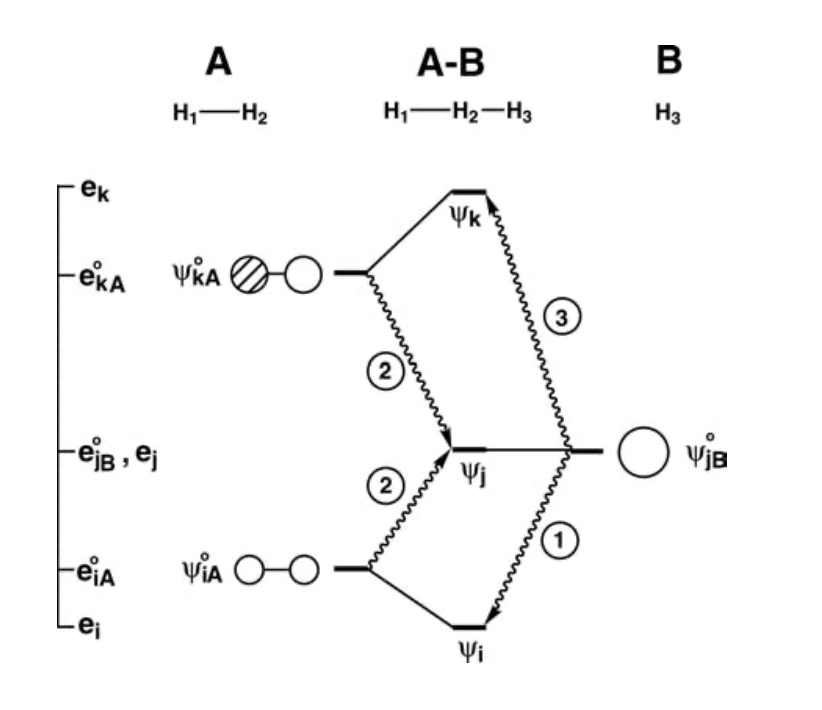
\includegraphics[width=4in]{F_three_orbital.png}
    \caption{Molecular Orbital diagram for the three orbital problem}
    \label{F:three_orbital}
\end{figure}

We use the perturbation theory result to obtain the approximate shape of the perturbed 
wavefunctions. We first focus on perturbed orbital $\psi_{i}$ derived from $\psi_{iA}$, 
using the assumed form of perturbation matrix, up to second order.
\begin{align}
    \psi_{i} &= 
    \left[ 1 -  \frac{(\tilde{H}_{ij} - \order{\varepsilon_i}{0}\tilde{S}_{ij})\tilde{S}_{ij}}{\order{\varepsilon_i}{0} - \order{\varepsilon_j}{0}} \right.
    \left. - \frac{1}{2} \left(\frac{\tilde{H}_{ij} - \order{\varepsilon_i}{0}\tilde{S}_{ij}}{\order{\varepsilon_i}{0} - \order{\varepsilon_j}{0}} \right)^2 \right] \psi_{iA}^0 \\ 
    &+ \left[ \frac{\tilde{H}_{ij}- \order{\varepsilon_i}{0} \tilde{S}_{ij}}{\order{\varepsilon_i}{0} - \order{\varepsilon_j}{0}} \right.
    + \left. \frac{(\tilde{H}_{ik}- \order{\varepsilon_i}{0} \tilde{S}_{ik})(\tilde{H}_{kj}- \order{\varepsilon_i}{0} \tilde{S}_{kj})}{(\order{\varepsilon_i}{0} - \order{\varepsilon_j}{0})(\order{\varepsilon_i}{0} - \order{\varepsilon_k}{0})} \right] \psi_{jB}^0  \\
    &+ \left[ \frac{\tilde{H}_{ik}- \order{\varepsilon_i}{0} \tilde{S}_{ik}}{\order{\varepsilon_i}{0} - \order{\varepsilon_k}{0}} \right.
    + \left. \frac{(\tilde{H}_{ij}- \order{\varepsilon_i}{0} \tilde{S}_{ij})(\tilde{H}_{jk}- \order{\varepsilon_i}{0} \tilde{S}_{jk})}{(\order{\varepsilon_i}{0} - \order{\varepsilon_k}{0})(\order{\varepsilon_i}{0} - \order{\varepsilon_j}{0})} \right] \psi_{kA}^0 
\end{align}
We further note that the second term in the bracket for $\psi_{jB}^0$ and the first term in the bracket for $\psi_{kA}^0$ vanish due to $\tilde{S}_{ik} = \tilde{H}_{ik} = 0$
so that the result can be reduced to 
\begin{align}
    \psi_{i} &= 
    \left[ 1 -  \frac{(\tilde{H}_{ij} - \order{\varepsilon_i}{0}\tilde{S}_{ij})\tilde{S}_{ij}}{\order{\varepsilon_i}{0} - \order{\varepsilon_j}{0}} \right.
    \left. - \frac{1}{2} \left(\frac{\tilde{H}_{ij} - \order{\varepsilon_i}{0}\tilde{S}_{ij}}{\order{\varepsilon_i}{0} - \order{\varepsilon_j}{0}} \right)^2 \right] \psi_{iA}^0 \\ 
    &+ \left[ \frac{\tilde{H}_{ij}- \order{\varepsilon_i}{0} \tilde{S}_{ij}}{\order{\varepsilon_i}{0} - \order{\varepsilon_j}{0}} \right] \psi_{jB}^0 
    + \left[ \frac{(\tilde{H}_{ij}- \order{\varepsilon_i}{0} \tilde{S}_{ij})(\tilde{H}_{jk}- \order{\varepsilon_i}{0} \tilde{S}_{jk})}{(\order{\varepsilon_i}{0} - \order{\varepsilon_k}{0})(\order{\varepsilon_i}{0} - \order{\varepsilon_j}{0})} \right] \psi_{kA}^0 \\
    &= (1 + \order{t_{ii}}{2}) \psi_{iA}^0 + \order{t_{ji}}{1} \psi_{jB}^0 + \order{t_{ki}}{2}\psi_{kA}^0
\end{align}

Let's consider the sign of these mixing coefficients, it can be seem that they mostly depend on the sign of the overlap integral $S_{ij}$ as well as the relative 
energy level between the orbitals. In the case of figure \ref{F:three_orbital}, we find the parameters:
\begin{equation}
    \tilde{S}_{ij}, \tilde{S}_{kj} > 0 
\end{equation}
and take $H_{\mu\nu} \propto (H_{\mu\mu} + H_{\nu\nu}) S_{\mu\nu} \propto - S_{\mu\nu}$ as well as $(H_{\mu\nu} - \varepsilon^0 S_{\mu\nu}) \propto - S_{\mu\nu} $
since the second term is relatively small. Now, we can determine the sign of the mixing coefficients:
\begin{align}
    \order{t_{ii}}{2} &= - [ (+) + (+) ] < 0 \\ 
    \order{t_{ji}}{1} &= \frac{(-)}{(-)} > 0 \\
    \order{t_{ki}}{2} &= \frac{(+)}{(+)} > 0
\end{align}
So that we find that both $\psi_{jB}^0$ and $\psi_{kA}^0$ mix positively into $\psi_{iA}^0$ in first order and second order. The obtained orbital 
can be approximately shown as in figure \ref{F:psi_i}. 
\begin{figure}[h!]
    \centering
    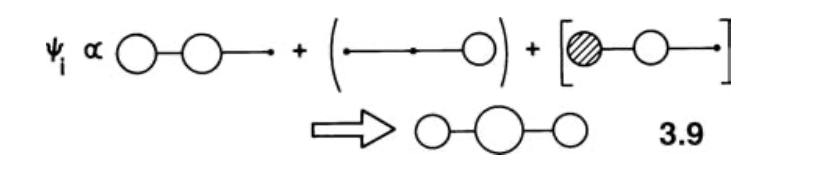
\includegraphics[width=4in]{F_psi_i.png}
    \caption{Orbital $\psi_{i}$}
    \label{F:psi_i}
\end{figure}

At this point, it is possible to point out a simple rule related to the sign of mixing coefficient 
for first order interaction, since it is simply given by the formula:
\[ t_{ji}^{(1)} = \frac{\tilde{H}_{ij}- \order{\varepsilon_i}{0} \tilde{S}_{ij}}{\order{\varepsilon_i}{0} - \order{\varepsilon_j}{0}}\] 
suppose that the orbitals are aligned so that $\tilde{S}_{ij}$ when they are brought together, we can 
see that:
\begin{itemize}
    \item The higher energies orbital mix \emph{into} the lower energy orbital with positive coefficients and,
    \item The lower energies orbital is substracted from the higher energy orbitals with a negative coefficients.
\end{itemize}

The other two orbitals can be obtained in the same fashion. The results are listed as follows:
\begin{align}
    \psi_{j} \approx \psi_{jB}^0 + |\order{t_{ij}}{1}| \psi_{iA}^0 - |\order{t_{kj}}{1}| \psi_{kA}^0 \\ 
    \psi_k \approx \psi_{kA}^0 - |\order{t_{jk}}{1}| \psi_{jB}^0 + |\order{t_{ik}}{2}| \psi_{iA}^0
\end{align}
where the sign correspond to the sign of the mixing coefficient $t$. The orbital are illustrated in figure \ref{F:psi_jk}.
\begin{figure}[h!]
    \centering
    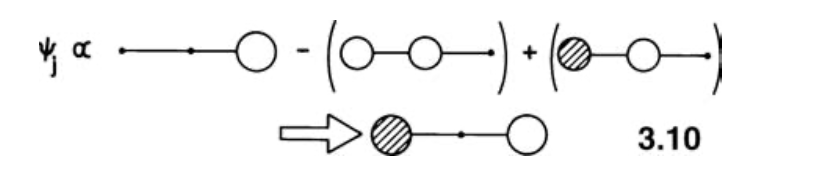
\includegraphics[width=4in]{F_psi_j.png}
    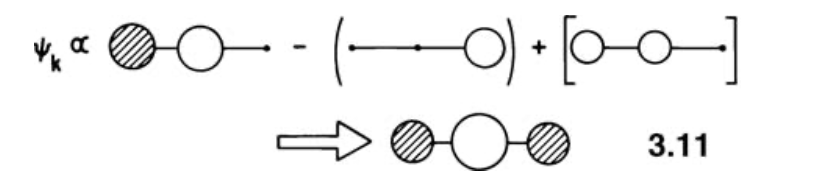
\includegraphics[width=4in]{F_psi_k.png}
    \caption{Orbital $\psi_{i}$ and $\psi_{k}$}
    \label{F:psi_jk}
\end{figure}


\end{document}
